\chapter{Utilizas triángulos: ángulos y relaciones métricas}

\section{Tipo de ángulos y relaciones entre ángulos}

Un ángulo es la parte del plano entre dos semirrectas con el mismo punto de
origen. La medida de este ángulo se llama amplitud. Un grado (sexagesimal)
es la amplitud de un ángulo igual a $\frac{1}{360}$ de la circunferencia.
Si los semirrectas no son coincidentes o alineadas, determinan dos ángulos, uno
convexo (el de menor amplitud) y otro cóncavo (el de mayor amplitud).

\begin{center}
\begin{tabular}{| c | c  | c |}
\hline
Tipo & Amplitud & \\
\hline
Ángulo nulo & $A = 0°$ & 
\begin{tikzpicture}
   \draw (0,0) -- (1,0);
 \end{tikzpicture} \\
\hline
Ángulo agudo & $0° < A < 90°$ &
 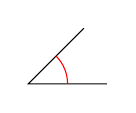
\begin{tikzpicture}
   \draw (1,0) -- (0,0) -- (0.707,0.707);
   \draw (.5,0) arc (0:45:.5)[color=red];
 \end{tikzpicture} \\
\hline
Ángulo recto & $A = 90°$ &
 \begin{tikzpicture}
   \draw (1,0) -- (0,0) -- (0,1);
   \draw (.2,0) -- (.2,.2) -- (0,.2)[color=red];
 \end{tikzpicture} \\
\hline
Ángulo obtuso & $90° < A < 180°$ &
 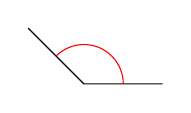
\begin{tikzpicture}
   \draw (1,0) -- (0,0) -- (-0.707,0.707);
   \draw (.5,0) arc (0:135:.5)[color=red];
 \end{tikzpicture} \\
\hline
Ángulo llano & $A = 180°$ & 
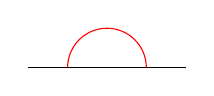
\begin{tikzpicture}
   \draw (1,0) -- (0,0) -- (-1,0);
   \draw (.5,0) arc (0:180:.5)[color=red];
 \end{tikzpicture}\\
\hline
Ángulo oblicuo & $A \neq 0°, 90°, 180°, 270°, 360°$ &\\
\hline
Ángulo completo o perigonal & $A = 360°$&
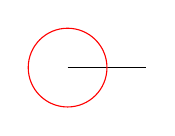
\begin{tikzpicture}
   \draw (0,0) -- (1,0);
   \draw (.5,0) arc (0:360:.5)[color=red];
 \end{tikzpicture} \\
\hline
\end{tabular}
\end{center}

\subsection{Ejercicio 1}

Indique el tipo de los ángulos de medidas siguientes:
35°, 180°, 45°, 200°, 90°, 350°, 0°, 100°.

\subsection{Definición}

Dos ángulos son complementarios si sus medidas suman 90°:

\begin{center}
 \begin{tikzpicture}
   \draw (0,0) -- (2,0);
   \draw (0,0) -- (1.7320,1);
   \draw (0,0) -- (0,2);
   \draw (0,.2) -- (.2,.2) -- (.2,0);
   \draw (.5,0) arc (0:30:.5)[color=red] node(A){};
   \draw (A) arc (30:90:.5)[color=blue];
 \end{tikzpicture}

\end{center}

Dos ángulos son suplementarios si sus medidas suman 180°:

\begin{center}
 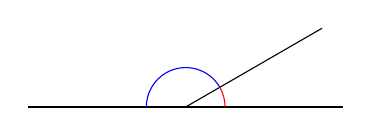
\begin{tikzpicture}
   \draw (0,0) -- (2,0);
   \draw (0,0) -- (1.7320,1);
   \draw (0,0) -- (-2,0);
   \draw (.5,0) arc (0:30:.5)[color=red] node(A){};
   \draw (A) arc (30:180:.5)[color=blue];
 \end{tikzpicture}
\end{center}

En la figura siguiente, los ángulos rojos son dichos opuestos por el vértice.
Son suplementarios del ángulo azul y entonces iguales:

\begin{center}
 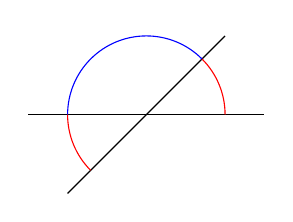
\begin{tikzpicture}
   \draw (-1.5,0) -- (1.5,0);
   \draw (-1,-1) -- (1,1);
   \draw (1,0) arc (0:45:1)[color=red] node(A){};
   \draw (A) arc (45:180:1)[color=blue];
   \draw (-1,0) arc (180:225:1)[color=red];
 \end{tikzpicture}

\end{center}


Consideramos dos rectas paralelas y una transversal a ellas. En la figura
siguiente, los ángulos de mismos colores son dichos correspondientes y tienen
la misma amplitud:

\begin{center}

 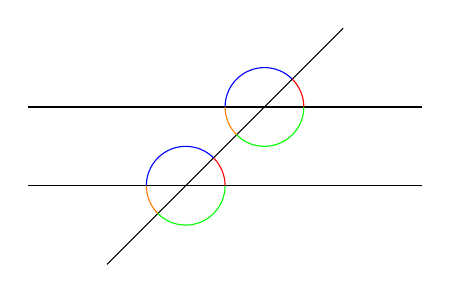
\begin{tikzpicture}
   \draw (0,0) -- (5,0);
   \draw (0,1) -- (5,1);
   \draw (1,-1) -- (4,2);
   \draw (3.5,1) arc (0:45:.5)[color=red] node(A){};
   \draw (A) arc (45:180:.5)[color=blue] node(B){};
   \draw (B) arc (180:225:.5)[color=orange] node(C){};
   \draw (C) arc (225:360:.5)[color=green];

   \draw (2.5,0) arc (0:45:.5)[color=red] node(AA){};
   \draw (AA) arc (45:180:.5)[color=blue] node(BB){};
   \draw (BB) arc (180:225:.5)[color=orange] node(CC){};
   \draw (CC) arc (225:360:.5)[color=green];

 \end{tikzpicture}

\end{center}

En la figura siguiente, los ángulos de mismos colores son dichos
alternos y tienen la misma amplitud:

\begin{center}

 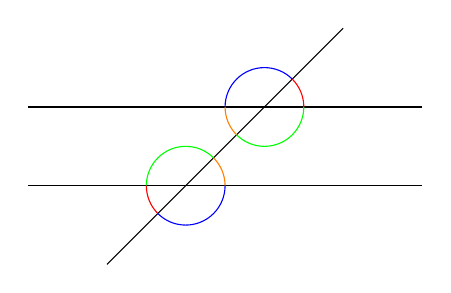
\begin{tikzpicture}
   \draw (0,0) -- (5,0);
   \draw (0,1) -- (5,1);
   \draw (1,-1) -- (4,2);
   \draw (3.5,1) arc (0:45:.5)[color=red] node(A){};
   \draw (A) arc (45:180:.5)[color=blue] node(B){};
   \draw (B) arc (180:225:.5)[color=orange] node(C){};
   \draw (C) arc (225:360:.5)[color=green];

   \draw (2.5,0) arc (0:45:.5)[color=orange] node(AA){};
   \draw (AA) arc (45:180:.5)[color=green] node(BB){};
   \draw (BB) arc (180:225:.5)[color=red] node(CC){};
   \draw (CC) arc (225:360:.5)[color=blue];

 \end{tikzpicture}

\end{center}

\subsection{Ejercicio 2}

Determine si los ángulos de amplitudes siguientes son complementarios,
suplementarios ningún de los dos:

\begin{itemize}
  \item ¿20° y 160°?
  \item ¿35° y 65°?
  \item ¿28° y 62°?
  \item ¿83° y 97°?
  \item ¿18° y 172°?
\end{itemize}

\subsection{Ejercicio 3}

Indique el ángulo complementario y suplementario de los ángulos siguientes de
amplitudes siguientes: 20°, 57°, 88°, 0°, 90°.

\subsection{Ejercicio 4}

Consideramos dos rectas paralelas y una transversal a ellas.
Indique los ángulos que son correspondiente y alternos con el ángulo rojo.
¿Si la amplitud del ángulo azul es 145°, cuales son las amplitudes de los otros?

\begin{center}

 \begin{tikzpicture}
   \draw (0,0) -- (8,0);
   \draw (0,2) -- (8,2);
   \draw (1,-1) -- (7,3);

   \draw (6.5,2) arc (0:35:1)[color=red] node(A){};
   \draw (A) arc (35:180:1)[color=blue] node(B){};
   \draw (B) arc (180:215:1)[color=green];

   \draw (3.5,0) arc (0:35:1)[color=purple];
   \draw (1.5,0) arc (180:215:1)[color=orange];

 \end{tikzpicture}

\end{center}

\section{Triángulos, lados y ángulos}

Podemos definir un (único) triángulo a partir de las medidas de sus lados
$a, b, c$ si y sólo si $c$ es el $a < b + c$, $b < a + c$ y $c < a + b$.

\begin{center}

 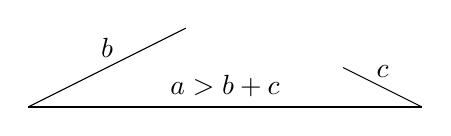
\begin{tikzpicture}
   \path (0,0) edge node[above]{$a > b + c$} (5,0) ;
   \path (0,0) edge node[above]{$b$} (2,1) ;
   \path (5,0) edge node[above]{$c$} (4,.5) ;
 \end{tikzpicture}

\end{center}

Un triángulo es escaleno, si todos sus lados tienen longitudes diferentes.
Un triángulo es isósceles si tiene dos lados iguales. Un triángulo equilátero
tiene sus tres lados iguales.

Podemos definir un triángulo a partir de las medidas de dos ángulas
$\alpha, \beta > 0$ si y sólo si $\alpha + \beta < 180°$. Obtenemos una
infinidad de triángulos con los mismos amplitudes si hacemos variar
proporcionalmente las longitudes de los lados. Si $\gamma$ es la
medida del tercer ángulo, tenemos
%%
$$
\alpha + \beta + \gamma = 180°
$$

Un triángulo es escaleno, si y solo si todos sus ángulos tienen amplitudes
diferentes.
Un triángulo es isósceles, si y solo si tiene dos ángulos de misma amplitud.
Es equilátero si y solo si tiene sus tres ángulos de misma amplitud, es decir
$\frac{180}{3} = 60°$.

Si una de los ángulo es recto (90°), el triángulo es dicho rectángulo. En
en otro caso es dicho oblicuángulo.

\begin{center}
 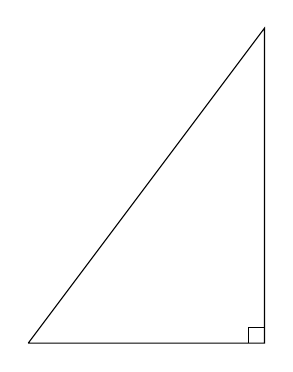
\begin{tikzpicture}
   \draw (0,0) -- (3,0) -- (3,4) -- (0,0);
   \draw (2.8,0) -- (2.8,.2) -- (3,.2);
 \end{tikzpicture}
\end{center}

Un triángulo es obtusángulo si uno de sus ángulos es obtuso (mayor de 90°) y
acutángulo si todos son agudos (menor de 90°).

\subsection*{Ejercicio 5}

Cuando es posible, dibuje un triángulo con las condiciones siguientes y indique
el tipo del triángulo.

\begin{itemize}
\item Triángulo de lados 3, 7, 3.
\item Triángulo de lados 3, 5, 3.
\item Triángulo de lados 3, 3, 3.
\item Triángulo de ángulos 90°, 75° y 25°.
\item Triángulo con dos lados de lado 7 formando un ángulo recto.
\item Triángulo de lados 6, 8, 10.
\item Triángulo con dos ángulos de medida 60°.
\item Triángulo con dos ángulos de medida 70° y 40°.
\item Triángulo de lados 7, 3, 10.
\item Triángulo con dos ángulos de medida 50° y 10°.
\item Triángulo con dos ángulos complementarios de medida diferentes de 45°.
\item Triángulo de lados 7, 8, 9.
\end{itemize}

\subsection{Ejercicio 6 (Tales)}

Consideramos un círculo de diámetro $[AB]$ y centro $O$. Sea $C$ otro punto
($\neq A,B$) sobre el círculo. ¿Cual es el tipo de los triángulos $OBC$ y
$OAC$? Si $\alpha = \widehat{BAC}$ y $\beta = \widehat{ABC}$ exprese el
ángulo $\widehat{BCA}$ en función de $\alpha, \beta$. Exprese la
suma de los ángulos del triángulo $ABC$ en función de $\alpha, \beta$. Deducir
que $ABC$ es rectángulo en $C$.

\section{Soluciones de los ejercicios}

\subsection*{Ejercicio 1}

agudo y oblicuo, llano, agudo y oblicuo, oblicuo, recto, oblicuo, nulo, obtuso y
oblicuo.

\subsection*{Ejercicio 2}

\begin{itemize}
  \item suplementario
  \item ningún de los dos
  \item complementario
  \item suplementario
  \item ningún de los dos
\end{itemize}

\subsection*{Ejercicio 3}

Las medidas de los ángulos complementarios son 70°, 33°, 2°, 90°, 0°.
Las medidas de los ángulos suplementarios son 160°, 123°, 92°, 90°, 180°.

\subsection*{Ejercicio 4}

El ángulo naranja es alterno con el ángulo rojo, el ángulo ṕurpuro es
correspondiente con el ángulo rojo. Los ángulos rojo y verde son opuestos
por el vértice y entonces iguales. Por la primera pregunta,
es también la medida de los ángulos naranja y ṕurpuro.

\subsection*{Ejercicio 5}

\begin{itemize}
\item No es posible por que $7 > 3 + 3$.
\item obtusángulo, isósceles, oblicuángulo.
\item acutángulo, equilatero, oblicuángulo.
\item No es posible por que $90 + 75 + 25 \neq 180$.
\item escaleno, rectángulo.
\item acutángulo, equilatero, oblicuángulo.
\item acutángulo, isósceles, oblicuángulo.
\item No es posible por que $10 = 3 + 7$.
\item obtusángulo, escaleno, oblicuángulo.
\item escaleno, rectángulo.
\item acutángulo, escaleno, oblicuángulo.
\end{itemize}

\subsection{Ejercicio 6 (Tales)}

$OBC$ y $OAC$ son isósceles por que $OA = OB = OC$ es el radio del círculo.
Entonces $\widehat{OAC} = \widehat{OCA} = \alpha$ y
$\widehat{OBC} = \widehat{OCB} = \beta$.

Tenemos $\widehat{BCA} = \alpha+\beta$ y
la suma de de los ángulos de $ABC$ es
$180° = \widehat{ABC} + \widehat{BCA} + \widehat{CAB} =
\beta + {(\alpha+\beta)} + \alpha = 2\left(\alpha+\beta\right)$.

Finalmente, $\widehat{BCA} = 90°$ y $ABC$ es rectángulo en $C$.
